\documentclass{article}
\usepackage{lipsum}
\usepackage{fancyhdr}
\usepackage[all]{xy}
\usepackage{amsmath, amsthm, latexsym, amssymb, graphicx,color,cite,mathabx,enumerate,mathrsfs}
\usepackage[left=2.0 cm,right=2.0cm,top=3cm,bottom=3cm]{geometry}
\pagenumbering{arabic}
\pagestyle{fancy}
\rhead{YOUR NAME}
\usepackage{dsfont}
\newtheorem{theorem}{Theorem}
\newtheorem{fact}{Fact}
\newtheorem{lemma}{Lemma}
\newtheorem{definition}{Definition}
\newtheorem{corollary}{Corollary}
\newtheorem{proposition}{Proposition}
\newtheorem{remark}{Remark}
\newtheorem{notation}{Notation}
\newtheorem{example}{Example}
\newtheorem{non-example}{Non-example}
\renewcommand{\Re}{\operatorname{Re}}%%redefined Re and Im
\renewcommand{\Im}{\operatorname{Im}}
\newcommand{\tr}{\operatorname{tr}}
\renewcommand{\det}{\operatorname{det}}
\newcommand{\cadlag}{\textit{c\'{a}dlag} }
\newcommand{\E}{\mathbb{E}}%notation for expectation
\newcommand{\unit}[1]{\overline{\underline{#1}}}%notation for the unit contraction function

\usepackage{amsmath}
%\usepackage{svgcolor}
\usepackage[svgnames]{xcolor}
\usepackage[framemethod=tikz]{mdframed}


\title{Euler-Lagrange Equations\\in\\Partial Differential Equations}
\author{Huan Q. Bui}
\date{May 18, 2019}
\begin{document}
\pagenumbering{roman}
\maketitle
\begin{center}
\includegraphics[scale=1]{Figure.eps}\\

Put your figure here.
\end{center}



\newpage
\tableofcontents
\newpage
\pagenumbering{arabic}
\section{Introduction}
\noindent Lorem ipsum dolor sit amet, consectetur adipiscing elit. Integer sollicitudin, orci vel fringilla sollicitudin, quam urna sodales elit, sit amet blandit tortor nunc imperdiet nulla. Nulla facilisi. Vestibulum non malesuada est, at viverra orci. In hac habitasse platea dictumst. Donec porta sollicitudin tortor viverra gravida. Aliquam vel tincidunt nisi. Vivamus pulvinar porta vehicula. Proin eget tincidunt tortor.

Pellentesque efficitur, est eget posuere bibendum, risus orci tincidunt felis, vel tempor risus ex et tellus. Praesent luctus malesuada augue, non faucibus nisl placerat finibus. Morbi convallis neque sit amet mattis pulvinar. Mauris rhoncus maximus arcu, quis commodo metus vulputate in. Donec congue lectus eget ligula placerat auctor. Proin nunc lectus, ultricies pellentesque tempor quis, sodales eu magna. Donec ante dui, rhoncus vel dui ac, ultricies viverra augue. Curabitur nibh ante, congue a lorem eu, hendrerit lacinia elit.

Duis interdum erat pharetra, rhoncus lectus consequat, bibendum lorem. Mauris lectus mi, varius et turpis nec, ullamcorper semper elit. Aenean efficitur faucibus dui id gravida. Suspendisse potenti. Fusce ullamcorper justo est, eu laoreet tortor efficitur non. Sed quis arcu vulputate, consectetur nisl at, consectetur massa. Duis quis ullamcorper libero, id convallis neque. Mauris risus lorem, vestibulum ut est dignissim, consequat laoreet tellus.

Duis hendrerit risus nec lacus aliquam, vel efficitur magna suscipit. Nunc vitae pretium turpis, non malesuada nibh. Aenean ac mauris nulla. Suspendisse fermentum libero in urna tincidunt convallis. Pellentesque rhoncus egestas nunc, vitae consequat lectus tincidunt a. Donec a faucibus purus. Mauris ornare erat a purus pellentesque blandit. Mauris in pulvinar sem, sed volutpat nulla. Vestibulum feugiat nisi ut vestibulum suscipit. Maecenas eget nisi condimentum, vulputate mauris sit amet, dignissim magna. Phasellus a turpis sit amet neque ornare iaculis. In a sodales felis. Donec sollicitudin lacus at lacus accumsan, sit amet condimentum lectus dapibus. Suspendisse potenti. Quisque et nulla lorem. We have

\begin{equation*}
e^{i\pi}+1=0.
\end{equation*}
The equation
\begin{equation}\label{eq:EulersEquation}
e^{it}=\cos(t)+i\sin(t)
\end{equation}
which holds for all $t\in\mathbb{R}$ shall be referred to again. In fact, the equation \eqref{eq:EulersEquation} is called Euler's identity.

\section{Functional Analysis}
Duis interdum erat pharetra, rhoncus lectus consequat, bibendum lorem. Mauris lectus mi, varius et turpis nec, ullamcorper semper elit. Aenean efficitur faucibus dui id gravida. Suspendisse potenti. Fusce ullamcorper justo est, eu laoreet tortor efficitur non. Sed quis arcu vulputate, consectetur nisl at, consectetur massa. Duis quis ullamcorper libero, id convallis neque. Mauris risus lorem, vestibulum ut est dignissim, consequat laoreet tellus.

Duis hendrerit risus nec lacus aliquam, vel efficitur magna suscipit. Nunc vitae pretium turpis, non malesuada nibh. Aenean ac mauris nulla. Suspendisse fermentum libero in urna tincidunt convallis. Pellentesque rhoncus egestas nunc, vitae consequat lectus tincidunt a. Donec a faucibus purus. Mauris ornare erat a purus pellentesque blandit. Mauris in pulvinar sem, sed volutpat nulla. Vestibulum feugiat nisi ut vestibulum suscipit. Maecenas eget nisi condimentum, vulputate mauris sit amet, dignissim magna. Phasellus a turpis sit amet neque ornare iaculis. In a sodales felis. Donec sollicitudin lacus at lacus accumsan, sit amet condimentum lectus dapibus. Suspendisse potenti. Quisque et nulla lorem. We have

\subsection{Semigroups and their infinitesimal generators}
\noindent Duis interdum erat pharetra, rhoncus lectus consequat, bibendum lorem. Mauris lectus mi, varius et turpis nec, ullamcorper semper elit. Aenean efficitur faucibus dui id gravida. Suspendisse potenti. Fusce ullamcorper justo est, eu laoreet tortor efficitur non. Sed quis arcu vulputate, consectetur nisl at, consectetur massa. Duis quis ullamcorper libero, id convallis neque. Mauris risus lorem, vestibulum ut est dignissim, consequat laoreet tellus.

Duis hendrerit risus nec lacus aliquam, vel efficitur magna suscipit. Nunc vitae pretium turpis, non malesuada nibh. Aenean ac mauris nulla. Suspendisse fermentum libero in urna tincidunt convallis. Pellentesque rhoncus egestas nunc, vitae consequat lectus tincidunt a. Donec a faucibus purus. Mauris ornare erat a purus pellentesque blandit. Mauris in pulvinar sem, sed volutpat nulla. Vestibulum feugiat nisi ut vestibulum suscipit. Maecenas eget nisi condimentum, vulputate mauris sit amet, dignissim magna. Phasellus a turpis sit amet neque ornare iaculis. In a sodales felis. Donec sollicitudin lacus at lacus accumsan, sit amet condimentum lectus dapibus. Suspendisse potenti. Quisque et nulla lorem. We have the following:

\begin{definition}\label{def:ImportantDefinition}
Suppose that $X$ is a Banach space and $D(A)\subseteq X$ is a linear subspace of $X$. By a linear operator $A$ on $X$ with domain $D(A)$, we mean a function $A:D(A)\rightarrow X$ that is $\mathbb{C}$-linear. We shall say that $A$ is densely defined if $D(A)$ is a dense subset of $X$ with respect to the norm topology.
\end{definition}

\begin{definition}[Closed operator]\label{def:AnotherImportantDefinition}
A linear operator $C$ on $X$ with domain $D(C)$ is said to be closed if for all $\{x_n\}_n\subseteq D(C)$ such that
\begin{equation*}
x_n\rightarrow x\hspace{1cm}\mbox{and}\hspace{1cm}Cx_n\rightarrow y
\end{equation*}
as $n\rightarrow \infty$, we have 
\begin{equation*}
x\in D(C)\hspace{1cm}\mbox{and}\hspace{1cm}Cx=y.
\end{equation*}
\end{definition}

Here is a remark:
\begin{remark}\label{rmk:Aremark}
It's silly to make a remark about a remark.
\end{remark}
Now I can talk about the remark, Remark \ref{rmk:Aremark} while refering to 
\begin{proposition}[Basic semigroup facts]\label{prop:basicsemigroupfacts}
Let $\{T_t\}_{t\geq 0}$ be a semigroup on $X$. 
\begin{enumerate}
 \item There are constants $C\geq 1$ and $\gamma\geq 0$ such that
\begin{equation*}
\|T_t\|_{op}\leq Ce^{t\gamma}
\end{equation*}
for all $t\geq 0$. 
\item For each $x\in X$, the map $t\rightarrow T_tx$ from $[0,\infty)$ into $X$ is continuous.
\end{enumerate}
\end{proposition}
\begin{proof}
$1.$ First we establish the existence of $C$. Suppose that for some sequence of non-negative real numbers $t_n\rightarrow 0$ we have $\|T_{t_n}\|_{op}\rightarrow \infty$. Then by the uniform boundedness principle, there is $x\in X$ for which
\begin{equation*}
\lim_{n\rightarrow\infty}\|T_{t_n}x\|=\infty.
\end{equation*}
This cannot be true in view of Property $iii$ of Definition \ref{def:ImportantDefinition}. Consequently, there must be $C\geq 1$ and $\delta>0$ for which
\begin{equation}\label{eq:bsgfact1}
\|T_t\|_{op}\leq C
\end{equation}
for all $t\in[0,\delta]$. Using the semigroup property, it follows that for any $t\geq 0$ and natural number $n$,
\begin{equation*}
T_{t}=T_{nt/n}=(T_{t/n})^n
\end{equation*}
and therefore
\begin{equation}\label{eq:bsgfact2}
 \|T_{t}\|_{op}\leq \|T_{t/n}\|_{op}^n.
\end{equation}
So for any $t\in[0,\infty)$ choose a natural number $n$ for which $(n-1)\delta\leq t< n\delta$. Combining \eqref{eq:bsgfact1} and \eqref{eq:bsgfact2} we have
\begin{equation*}
\|T_t\|_{op}\leq \|T_{t/n}\|_{op}^n\leq C^n=CC^{n-1}\leq CC^{t/\delta}=Ce^{\gamma t}
\end{equation*}
 where $\gamma=(\log(C))/\delta\geq 0$. This proves the first part of the proposition.

For the second, observe that for any $x\in X$, $t\in[0,\infty)$ and $h>0$,
\begin{equation*}
\|T_{t+h}x-T_tx\|=\|T_t(T_hx-x)\|\leq Ce^{\gamma t}\|T_hx-x\|
\end{equation*}
where we have used the semigroup property. By an appeal to Property $iii.$ of Definition \ref{def:AnotherImportantDefinition}, the proof is complete. You can also cite references \cite{HB98} and \cite{CA} here. The references  \cite{MSW00} and  \cite{Rei91}might also be useful.
\end{proof}

\footnotesize
 \begin{thebibliography}{99}

\bibitem{HB98} Huynen, M.~A. and Bork, P. 1998. Measuring genome evolution. {\em
Proceedings of the National Academy of Sciences USA}
  95:5849--5856.

\bibitem{CA} Caprara, A. 1997. Sorting by reversals is difficult. In: {\em
Proceedings of the First Annual International Conference on Computational
Molecular Biology (RECOMB 97),} New York: ACM.  pp. 75-83.

\bibitem{MSW00}McLysaght, A., Seoighe, C. and Wolfe, K.~H. 2000. High frequency
of inversions during eukaryote gene order evolution.     In Sankoff, D. and
Nadeau, J.~H., editors, {\em Comparative Genomics},  Dordrecht, NL: Kluwer
Academic Press. pp. 47--58.

\bibitem{Rei91} Reinelt, G. 1991. {\em The Traveling Salesman - Computational
Solutions for TSP Applications.} Berlin: Springer Verlag.

\end{thebibliography}



%\bibliographystyle{acm} % (uses file "plain.bst")  %You can also use your own .bib file
%\bibliography{refs}
\end{document}